\documentclass[tikz,border=5pt,12pt]{standalone}
\usepackage{tikz}
\usetikzlibrary{calc}
\usepackage{pgf,xcolor}
\usepackage{eulervm}
\usepackage{booktabs,rotating,multirow,caption}
\usepackage{makecell}
\usetikzlibrary{decorations.pathreplacing}
\usetikzlibrary{backgrounds}
\newcommand*\packet[1]{\tikz[baseline=(char.base)]{
            \node[thick,fill=white,shape=rectangle,draw,inner sep=2.5pt] (char) {#1};}}
\begin{document}
\begin{small}
{\sffamily
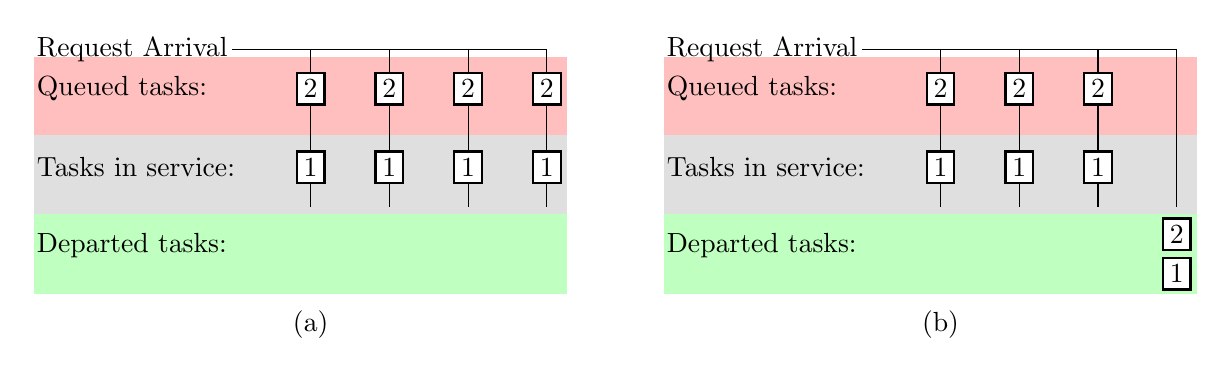
\begin{tikzpicture} 
\draw [fill=red!25,red!25] (-3.5,-0.1) rectangle (3.25,-1.1); 
\draw [fill=gray!25,gray!25] (-3.5,-1.1) rectangle (3.25,-2.1); 
\draw [fill=green!25,green!25] (-3.5,-2.1) rectangle (3.25,-3.1); 
\draw (-1,0) -- (3,0);
%service
\draw (0,0) -- (0,-2);
\draw (1,0) -- (1,-2);
\draw (2,0) -- (2,-2);
\draw (3,0) -- (3,-2);
%
\node at (0,-1.5) {$\packet{1}$};
\node at (1,-1.5) {$\packet{1}$};
\node at (2,-1.5) {$\packet{1}$};
\node at (3,-1.5) {$\packet{1}$};
%
\node at (0,-0.5) {$\packet{2}$};
\node at (1,-0.5) {$\packet{2}$};
\node at (2,-0.5) {$\packet{2}$};
\node at (3,-0.5) {$\packet{2}$};
%
\node [right] at (-3.6,0) {Request Arrival};
\node [right] at (-3.6,-.5) {Queued tasks:};
\node [right] at (-3.6,-1.5) {Tasks in service:};
\node [right] at (-3.6,-2.5) {Departed tasks:};
%
\node at (0,-3.5) {\normalsize (a)};
%
%\hspace{1cm}
\begin{scope}[xshift=8cm]
\draw [fill=red!25,red!25] (-3.5,-0.1) rectangle (3.25,-1.1); 
\draw [fill=gray!25,gray!25] (-3.5,-1.1) rectangle (3.25,-2.1); 
\draw [fill=green!25,green!25] (-3.5,-2.1) rectangle (3.25,-3.1); 
\draw (-1,0) -- (3,0);
% 
\draw (0,0) -- (0,-2);
\draw (1,0) -- (1,-2);
\draw (2,0) -- (2,-2);
\draw (3,0) -- (3,-2);
% waiting
% in service
\node at (0,-0.5) {$\packet{2}$};
\node at (1,-0.5) {$\packet{2}$};
\node at (2,-0.5) {$\packet{2}$};
\node at (0,-1.5) {$\packet{1}$};
\node at (1,-1.5) {$\packet{1}$};
\node at (2,-1.5) {$\packet{1}$};
% departed
\node at (3,-2.35) {$\packet{2}$};
\node at (3,-2.85) {$\packet{1}$};
%
\node [right] at (-3.6,0) {Request Arrival};
\node [right] at (-3.6,-.5) {Queued tasks:};
\node [right] at (-3.6,-1.5) {Tasks in service:};
\node [right] at (-3.6,-2.5) {Departed tasks:};
%
\node at (0,-3.5) {\normalsize (b)};
\end{scope}
\end{tikzpicture}
}\end{small}
\end{document}